\chapter{IT valitsemine}
\section{Parimatest praktikatest}
\label{sec:governance:bp}
IT valdkonnas on käibel suur hulk kõivõimalikke metoodikaid ja raamistikke. Osa neist on ühel või teisel viisil kogumid parimatest praktikatest: grupp ettevõtteid on kokku leppinud, et mingisugune konkreetne viis mingisugust konkreetset probleemi lahendada on parim. Sellised on näiteks ITIL\index{ITIL} ja TOGAF\index{TOGAF} aga ka PMBOK\index{PMBOK}. Teataval määral on ka käesolev kogumik - kuigi tugineb vaid ühele inimesele - samast puust. 

Kindlasti on parimatel praktikatel oma väärtus, tegemist on ju õitsva äriga. ITIL annab väga hea ülevaate erinevatest IT juhtimisega seotud valdkondadest, PMBOK teeb sama projektijuhtimisega. Samas tuleb neisse suhtuda teatava ettevaatusega. Asi on selles, et parim praktika on tahes tahtmata keskmine. Leitakse hulk viise probleemi lahendada ning mõõdetakse nende edukust. Raamistikku jõuab miski, mis on nii laialt levinud kui edukas. Kuid organisatsioon, mis järgib keskmisi praktikaid saab paratamatult olla vaid keskmine. Samuti ei tähenda mõne praktika populaarsust, et tegemist on \emph{parima} praktikaga\sidenote{\quote{If majority is always right - let's eat shit... millions of flies can't be wrong.}\\Waldemar Łysiak}. Tegu on vaid parima teadaoleva praktikaga valimis. Kui suur hurk turuosalisi teeb näiteks konfiguratsioonjuhtimist ühel viisil, siis ei saa konfiguratsioonijuhtimine pakkuda ühele neist võimalust eristuda. 

Veelgi enam, seda keskmist ei olegi olemas\cite{averages}. On hulk organisatsioone, mis järgivad \emph{igaüht} neist praktikatest kuid ei ole organisatsiooni, mis järgib neist \emph{kõiki}. Ei ole mõistlik üritada olla nagu teised, sest, paradoksaalselt, mitte keegi ei ole selline nagu teised. Tuleks üritada leida lahendus oma probleemile ning määratleda just konkreetsele organisatsioonile sobiv tasakaal standardsete strateegiliste eeliste vahel.

Loomulikult on hulk valdkondi, kus eristuma ei peagi, mille kallal pea murdmine ei loo piisavalt väärtust. Kuid tänapäeval on üha väiksem hulk neist infotehnoloogias sest efektiivset eristumisvõijust otsitakse järjest enam just ITst.

\section{Poliitikavastasus. Hundid ja jänesed}
\index{Poliitikavastasus}

Kujutlegem lihtsat ökosüsteemi, mis koosneb huntidest ja jänestest. Hundid söövad jäneseid, jänesed elavad õhust ja armastusest (mida mõlemat on piisavalt). Loomade omavahelisi seoseid illustreerib joonis \ref{fig:wolves}. Oletagem, et meil on soov tõsta huntide arvukust. Seepärast tuuakse mujalt ja lastakse metsa lahti viis emast ja viis isast hunti. Mis juhtub? 
\begin{itemize}
	\item Huntide arvukus tõuseb kümne lisandunud hundi võrra
	\item Kuna kümme lisandunud hunti tahavad süüa, siis väheneb jäneste arvukus. Ajaühikus ära söödavate jäneste hulk ju suureneb
	\item Kuna jäneseid on vähem, väheneb ka jäneste juurdekasvu kiirus. Ära söödud jänesed ju uusi jäneseid ei tee. Samuti tahavad uued hundid ka homme süüa
	\item Seega hakkab jäneste arvukus vähenema
	\item Misjärel hakkavad hundid nälga jääma, sest kõigile enam jäneseid ei jagu
	\item Mistõttu saavad hundid vähem järglasi ja langeb nende juurdekasvu kiirus
	\item Kuna hundid surevad vanadusse ikka sama tempoga, hakkab huntide arvukus vähenema
	\item Kui huntide arvukus on jõudnud esialgsele tasemele, on kõigile jälle piisavalt jäneseid 
\end{itemize}

\begin{marginfigure}
		\begin{center}
		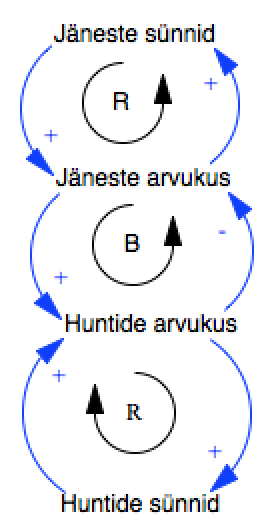
\includegraphics[width=.7\linewidth]{hundid.png}
		\caption{Huntide ja jäneste arvukuse seos}
		\label{fig:wolves}
		\end{center}
	Huntide ja jäneste arvukuse seos. Nii huntide kui jäneste puhul viib rohkem loomi rohkemate sündide ja seega rohkemate loomadeni. Kuid huntide arvukuse kasv viib alla jäneste arvukuse ning jäneste arvukuse langus viib alla huntide arvukuse.
\end{marginfigure}

Nii taastub esialgne olukord, algne huntide lisamine ei ole andnud soovitud tulemust. Huntide arvukus võiks tõusta hoopis tõstes jäneselaste arvu jäneseperekonnas ehk nende juurdekasvu kiiruse tõstmisega. 

\section{Inimeste valitsemine}
Valitsemise üsna lahutamatu osa on paraku vajadus inimesed organisatsioonist eemaldada. Jättes kõrvale juriidilised ja muud nüansid, on oluline aru saada, et mõtteliidri (\emph{thought leader}) lahkumine on meeskonna dünaamika jaoks oluline sündmus. Samuti on oluline mõista, et tegu on vältimatu protsessiga, mis seega on mõistlik läbi viia kontrollitult ja minimaalsete kadudega. Järgnevas selleks mõned näpunäited: 

\begin{itemize}
	\item Vii inimene organisatsioonist välja enne, kui tema vastuolud muutuvad meeskonna vastuoluks. Definistiooni järgi inimesed järgnevad liidrile ning kui tollel on kellegagi vastuolud, kanduvad nood paratamatult varem või hiljem meeskonda. Kui hiljaks jääda lahkuvad (või tuleb vastuseisu tõttu eemaldada) ka teised tiimi liikmed peale juhi. Nii võib oskamatu käitumisega vallandada lumepalliefekti, mis organisatsiooni kiiresti ajudest tühjendab.
	\item Väike (!) hulk võtmeisikuid peab plaanist ette teadma, sealhulgas muidugi ka eemaldatav ise. Nii on neil ühest küljest võimalik tulevaseks kriisiks valmistuda kuid teisalt saab nii vältida emotsionaalset avalikku käitumist ning muidu üllatusi. Etteteatamisaeg võib ulatuda mõnest päevast mõne tunnini. Pikem aeg tekitab permanentse kriisi olukorra ja kommunikatsioon väljub kontrolli alt
	\item Kommunikatsiooni kolm sammu. Kõik sammud läbitakse väga lühikeste (kõige rohkem mõned tunnid) intervallidega vältimaks uudiste lekkimist (ingl. \emph{techcrunch meltdown} tuntud tehnoloogiauudiste portalli järgi) ning minimeerimaks kriisi kestvust. 
		\begin{enumerate}
			\item "Vanaisa"\footnote{Juhi juht. Selles kontekstis isik, kes teeb otsuse inimene välja viia.} teade. Nii antakse teada, kes olukorda kontrollib. Sisaldab
				\begin{itemize}
					\item Kes lahkub millal ja miks. Tekst olgu viisakas, inimesed kas teavad niigi või suudavad ridade vahelt lugeda
					\item Mis juhtub järgmisena ja millal. Inimestele ei meeldi ebakindlus, hirmud tuleb maha võtta. Oluline punkt siin: kes ja millal asendab lahkuja?
					\item Muutused organisatsiooni toimimises. Lahkuja oli kindlasti osaline mingites äriprotsessides (koodi ülevaatused, tarnete vastu võtmine jms.), kuidas need edasi toimima hakkavad?
				\end{itemize}
			\item Lahkuja teade. Tavaliselt suunatud lähematele kolleegidele. Võib olla suhteliselt otsekohene aga kui on karta midagi mürgist, võib (viisakalt) paluda teksti kooskõlastamist
			\item Avalik teade. Kui vähegi usutav, võiks tekst olla kiitvas, positiivses ja tänulikus toonis. Kui mitte, siis lakooniline kuiv tekst.
		\end{enumerate}
\end{itemize}

\section{Ressursijuhtimine}
Järgnev on üks võimalik vaade asjadele: selgesti on avaliku- ja erasektori suhtumine rahasse erinev. Ainus põhjus, miks maksumaksja riigile raha annab, on, et selle raha eest osutataks avalikku teenust. Kui nüüd riik korjab raha kokku, kuid selle eest mõistlikku avalikku teenust ei osuta (ka reservide kogumine on avalik teenus), siis on tegu maksumaksja asjatu koormamisega. Erasektoris jaotatakse kasum omanike vahel, riigis selle mehhanismi ekvivalenti ei eksisteeri. Järelikult on erasektoris pigem surve raha mitte kulutada samas kui riigisektoris on pigem surve raha eest võimalikult palju teenust osutada.  

\section{Surnumere efekt}
Miks on Surnumeri soolane? Põhjus on lihtne: sinna lisandub küll suhteliselt soolast vett aga füüsikaseaduste tõttu aurab ära  vaid puhas $H_2O$. Nii võib kergesti juhtuda ka organisatsioonidega\sidenote{Loe lähemalt \url{http://brucefwebster.com/2008/04/11/the-wetware-crisis-the-dead-sea-effect/}}, eriti IT omadega. Lühidalt öeldes, organisatsiooni sisenevate ja sealt väljuvate inimeste talendi, hariduse, suhtumise, kogemuse ja oskuste tase ei lange kokku. Värvata õnnestub tõenäoliselt suhteliselt normaaljaotuse lähedast kontingenti kuid lahkuvad reeglina paremad. Ja nii tekib tagasiside: mida hullem on olukord organisatsioonis, seda nõrgemaid kandidaate õnnestub värvata, seda kiiremini filtreeruvad välja halvimatest parimad ja seda hullem on olukord. 

Kuidas tsükkel tekib ning kuidas sellest vabaneda? Tegu on olemuselt juhtimisprobleemiga. Kui vesi soolaseks läheb, on keegi on kuskil teinud juhtimisvea. Kuid käivitajaks võib olla ka viga personalitöös\index{Personal}. Näiteks võib kiire laienemise käigus organisatsiooni sisse tulla olemasolevatest oluliselt nõrgemaid inimesi või on kasutusel ebakompetentsuse suhtes tolerantne hindamissüsteem. Kuidas ka ei oleks, on oluline pidada silmas nii tulijate kui lahkujate oskusi. Kui me kaotame rohkem nutikaid inimesi (näiteks tiheda turusituatsiooni tõttu), peame ka palkamise sinnapoole kallutama. Vatupidine olukord - kaotame pigem keskmisest vähemnutikaid - võib tunduda isegi soovitavana kuid ka siin on omad ohud. Vaid staaridest koosnevad meeskonna koos hoidmine nõuab oluliselt kõrgemat juhtimiskompetentsi ning kindlasti tuleb silmas pidada ka palgataseme mõju ärimudelile.

Eriti sagedasti võib surnumere laadset mõistuslikku elu mitte toetavat keskkonda leida riigiasutuste IT-osakondades. IT organisatsioonid on efektile suhteliselt vastuvõtlikumad, kuna seal on isikliku panuse ja tulemuse seos tugev, tööjõuturgu teeb pakkuja ning inimeste omavahelised suhted on tihedad. Teisalt on riigiasutuses tavaliselt suhteliselt jäigad personaliga seotud reeglid, mis teevad inimestest organisatsiooni initsitatiivil vabanemise keeruliseks. 

\section{Protsesside juhtimine}
\subsection{Organisatsiooni kiirendamine}
Suurepärane näide organisatsiooni kiirendamisest on Singapur. Joonisel \ref{fig:kasv} on toodud viie riigi GNI aastatel 1995 kuni 2012. On näha, kuidas USA, Eesti, Läti ja Vene Föderatsioon kasvavavad suuresti samas rütmis, kuigi absoluutnumbrites on USA teistest kaugel ees. Singapur aga on suutnud aastast 2002 näidata teistest oluliselt kiiremat kasvu. Isegi arvestades 2008. aasta kriisi mõju, on kasv teistest oluliselt kiirem. Lühike järeldus joonisest on, et ühel või teisel viisil on Singapur suutnud mitte ainult kasvada, vaid kasvada teistest kiiremini. Kui Eesti aga ka jätkab senist stabiilset kasvu, ei õnnestu meil ilmselt kunagi USAle järele jõuda. 

\TODO Korralik joonis. Sama stiil, kui vigade graafik

\begin{figure}[h]
	\begin{center}
		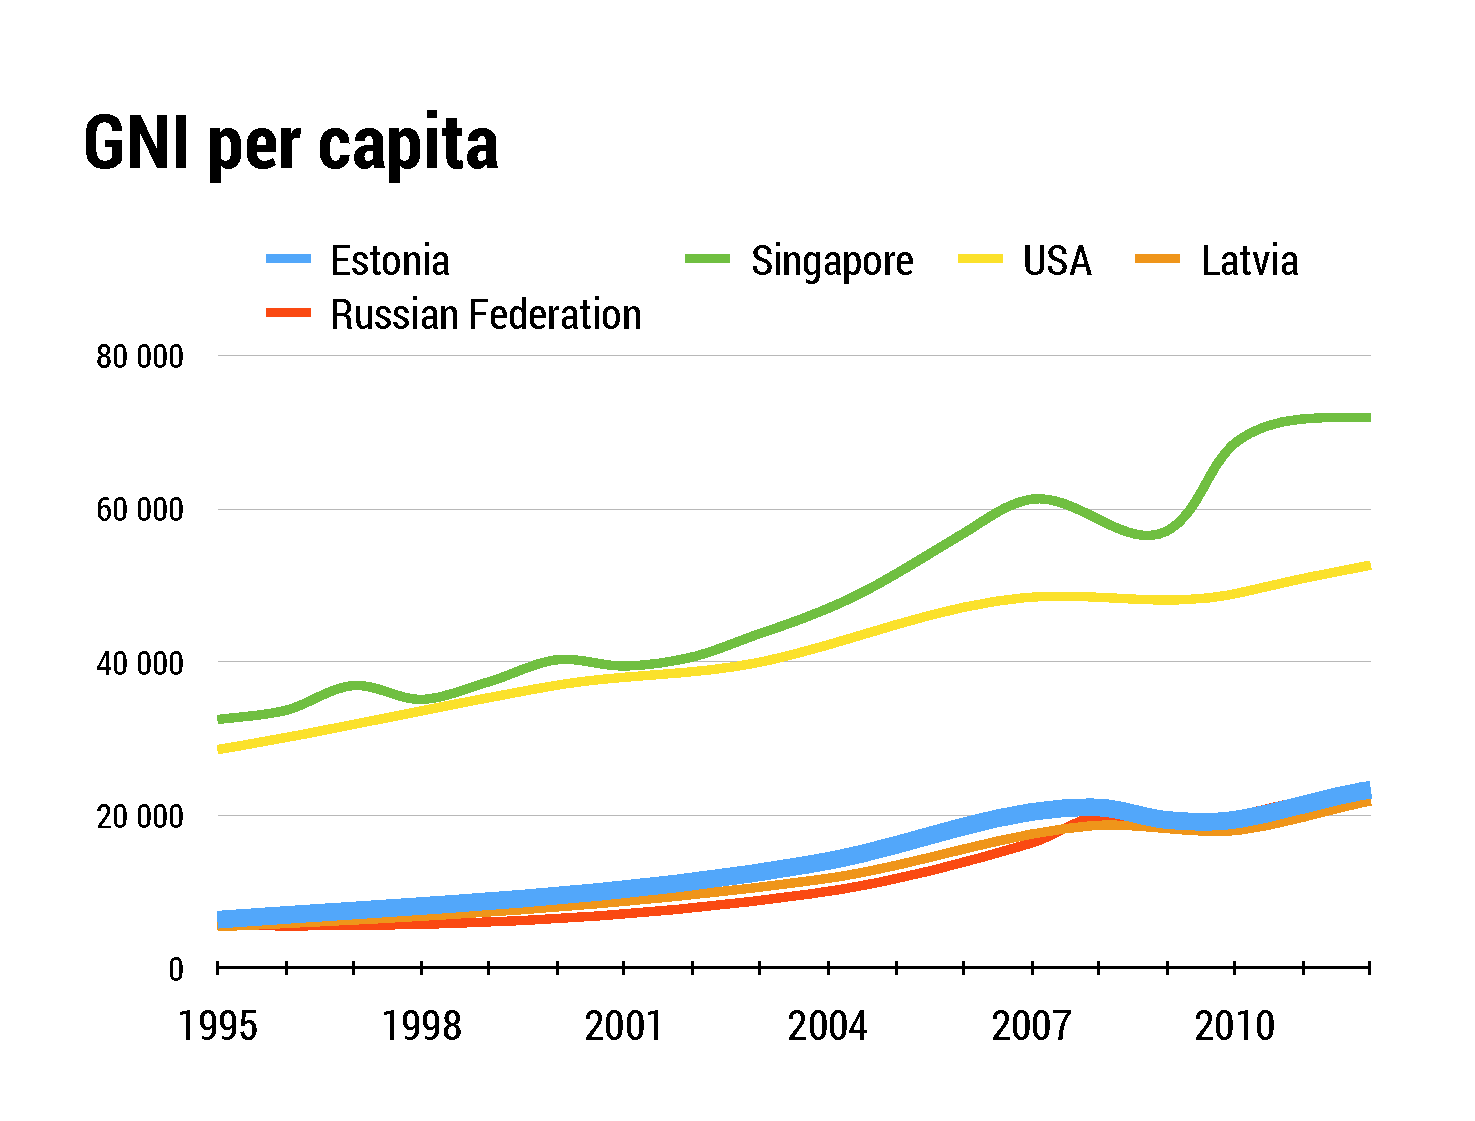
\includegraphics[width=\textwidth]{kasv.pdf}
		\caption{Riikide GNI võrdlus. Maailmapanga andmed.}
		\label{fig:kasv}
	\end{center}
\end{figure}

\subsection{Arenduse ootejärjekorra juhtimine}
Infotehnoloogia on tavaliselt põimunud sügavale organisatsiooni protsessidesse. Samuti on IT peamine protsesside efektiivistamise vahend. Järelikult on igas organisatsioonis suur hulk erinevaid arendusvajadusi. Samas on ressursid alati piiratud\footnote{Rangelt võttes võib probleemiks olla ka võimekus ressursside omavaheline vahetus. Näiteks on suurettevõtetes või avalikus sektoris tihti piiratud täistööajaga töötajate hulk, samuti võib saadaolev finantseering olla seotud pirangutega (selle kulutamine teatud riigis või teatud tegevusteks)} ning seega ületab organisatsiooni arendusvajadus reeglina IT-organisatsiooni võimekust seda vajadust täita\footnote{Vt. ka lõik \ref{sec:kulud} organisatsiooni võimekuse arengu kohta}. Järelikult kerkib küsimus tööülesannete järjestamisest. Mis järjekorras töid ette võtta?

Ootejärjekorral on järgnevad omadused:
\begin{itemize}
	\item Kuna töid tekib definitsiooni järgi kiiremini, kui neid täita suudetakse, siis järjekord kasvab. Kui vannist voolab vesi aeglasemalt, kui seda sinna lisandub, hakkab vee tase tõusma
	\item Mida pikem on ootejärjekord, seda paindumatum on organisatsioon. Kui järjekorras on x aasta jagu projekte, siis jõuab järjekorra viimane tegemisse kõige kiiremini x aastaga
	\item Kuna organisatsiooni äritulemuste saavutamine sõltub sageli ITst, eksisteerib ootejärjekorrale tugev poliitiline surve. Otsus mõnda projekti teha ja teist mitte võib omada mõne osalise jaoks omada isiklikku väljundit tulemustasu näol
\end{itemize}

Et ootejärjekord on pikk, tuleb ühel või teisel viisil sealt kas projekte välja jätta või vähendada organisatsiooni võimekust sinna asju lisada. Et otsused on seotud konfliktiga, minnakse sageli just ootejärjekorra barjääri tõstmise teed. Oma rolli mängib siin ka soov olemasolevat võimalikult efektiivselt kasutada suunates klienti võimalikult põhjalikku eeltööd tegema. IT kliendiks oleva keskastme juhi vaatenurgast vaadates tekib nii olukord, kus tema (organisatsiooni perspektiivist väheoluline, kuid tema jaoks kriitiline) arendusvajadus vajab ebaproportsionaalselt palju panust ning omab ikkagi väikest shanssi töösse minna. Eriti drastiline on probleem harukontorite puhul, millede probleemistikust ei pruugi lõpuni aru saada ka peakontori inimesed. Kui nüüd tollel juhil on initsiatiivi, juhtub tavaliselt üks kahest. Kui käepärast on krediitkaart, siis võidakse probleemi lahendamiseks hankida marginaalse hinna eest teenust mõnelt SaaS\footnote{\emph{Software as a Service} tarkvara kui teenus. Lahendus, kus tarkvara hallatakse keskselt ning lõppkasutaja maksab teenuse eest perioodiliselt proportsionaalselt teenuse kasutamisega} pakkujalt. Mispuhul tekib reeglina kohe riskijuhtimislik probleem sest kaob kontroll organisatsiooni andmete üle. Kui aga käepärast on IT-kompetentsi kas Exceli makrode või PHP tundja näol, luuakse tõenäoliselt kohalik infosüsteem. Sedalaadi infosüsteem ei vasta tavaliselt ühelegi keskse IT standardile, muutub ühel hetkel tellija jaoks kriitiliseks, kaotab oma ainsa arendaja (vahel kõike korraga) ning paneb keskse IT fakti ette: üle tuleb võtta dokumenteerimata, ebaturvaline ja profiilist välja jääv ärikriitiline tehniline lahendus. Tekitatud pusa ümber kirjutamiseks (kui isegi leidub keegi, kes suudaks sellise ülesande pädevalt püstitada) reeglina finantseeringut leida ei õnnestu. 

Taoliste olukordade vältimiseks on kriitiline, et järjekorrast projektide välja jäätmine oleks põhjalikult dokumenteeritud kui \enquote{sellega-me-ei-tegele-siin-majas} otsus ning et eksisteeriks ülevaade barjääri taga toimuvast. Samuti võib soovitada eraldi protsessi väikesemahulisteks arendusteks, mille abil on võimalik väikesed kuid olulised asjad tehtud saada. Tavaliselt on abi ka heast suhtest klientorganisatsiooni kõigi osadega, siin on abiks tugev ning suhtlemisaldis valdkonnajuht.

\TODO Faktorid, mis tekitavad tagasiside ootejärjekorraga:
\begin{itemize}
	\item Programmeerija context switch
	\item Paberimäärimine
	\item Isearendus
	\item Mikrojuhtimine
	\item Viide arhetüübile
\end{itemize}

\section{Küsimused aruteluks}
\subsection{Milline on põhimõtteline vahe IT juhtimise ja IT valitsemise vahel?}
Leadership vs. Management.

\subsection{Kuidas ja miks mõõta programmeerija tulemust?}
Auditooriumist
\begin{itemize}
	\item Kvaliteet
	\item Ajahinnangute hajuvus
\end{itemize}

Juhtum projektide boonustega, \enquote{saad, mida mõõdad}.

\subsection{Mida teha, kui klient ei kuula?}
Auditooriumist: karjuda. Kirjuta lahti põhimõttelise väärtuskonflikti küsimus. Newtoni essee lõik. 

\section{Lahti kirjutada}
Dropboxi ja infohalduse probleem. Dropboxi ei saa kinni panna, guerilla IT. Hall IT tekib kindlasti, kui teenus ei rahulda. Kätt ei saa ette panna.
